
\documentclass[a4paper,10pt,fleqn, twocolumn]{IEEETran}
\usepackage{amsfonts}
\usepackage{amsthm}
\usepackage{graphicx}
\usepackage{fancyhdr}

\newtheorem{Prop}{Proposition}
\newtheorem{lemma}{Lemma}


\setlength{\parindent}{3em} \setlength{\oddsidemargin}{0in}
\setlength{\textwidth}{6.5in} % sets 1in left and right margins
\setlength{\topmargin}{0.20in} % change to 0.2in for regular latex
%\setlength{\headheight}{0in}
%\setlength{\footheight}{0.5in}
\setlength{\footskip}{0.5in}
\setlength{\textheight}{9.0in} %sets 1in top and bottom margins
\renewcommand{\baselinestretch}{1} %set to 1.5 for double spacing.

\newcommand{\br}{{\mathbf r}}
\newcommand{\bA}{{\mathbf A}}
\newcommand{\ba}{{\bf a}}
\newcommand{\bb}{{\bf b}}
\newcommand{\bc}{{\bf c}}
\newcommand{\bC}{{\bf C}}
\newcommand{\bg}{{\bf g}}
\newcommand{\bG}{{\bf G}}
\newcommand{\bd}{{\bf d}}
\newcommand{\be}{{\bf e}}
\newcommand{\bq}{{\bf q}}
\newcommand{\bs}{{\bf s}}
\newcommand{\bm}{{\bf m}}
\newcommand{\bn}{{\bf n}}
\newcommand{\bu}{{\bf u}}
\newcommand{\bv}{{\bf v}}
\newcommand{\bw}{{\bf w}}
\newcommand{\bx}{{\bf x}}
\newcommand{\by}{{\bf y}}
\newcommand{\bz}{{\bf z}}
\newcommand{\bbf}{{\bf f}}
\newcommand{\bE}{{\bf E}}
\newcommand{\bF}{{\bf F}}
\newcommand{\bL}{{\bf L}}
\newcommand{\bM}{{\bf M}}
\newcommand{\bN}{{\bf N}}
\newcommand{\bS}{{\bf S}}
\newcommand{\bT}{{\bf T}}
\newcommand{\bD}{{\bf D}}
\newcommand{\bX}{{\bf X}}
\newcommand{\bP}{{\bf P}}
\newcommand{\bQ}{{\bf Q}}
\newcommand{\bI}{{\bf I}}
\newcommand{\bR}{{\bf R}}
\newcommand{\bU}{{\bf U}}
\newcommand{\bV}{{\bf V}}
\newcommand{\bW}{{\bf W}}
\newcommand{\bY}{{\bf Y}}
\newcommand{\bZ}{{\bf Z}}
\newcommand{\bJ}{{\bf J}}
\newcommand{\bB}{{\bf B}}
\newcommand{\bzero}{{\bf 0}}
\newcommand{\bgamma}{{\mbox {\boldmath $\gamma$}}}
\newcommand{\btheta}{{\mbox {\boldmath $\theta$}}}
\newcommand{\bLambda}{{\mbox {\boldmath $\Lambda$}}}
\newcommand{\bPsi}{{\mbox {\boldmath $\Psi$}}}
\newcommand{\bPhi}{{\mbox {\boldmath $\Phi$}}}
\newcommand{\bcA}{{\mbox {\boldmath ${\cal A}$}}}
\newcommand{\bcB}{{\mbox {\boldmath ${\cal B}$}}}
\newcommand{\bcC}{{\mbox {\boldmath ${\cal C}$}}}
\newcommand{\bcD}{{\mbox {\boldmath ${\cal D}$}}}
\newcommand{\bcF}{{\mbox {\boldmath ${\cal F}$}}}
\newcommand{\bcN}{{\mbox {\boldmath ${\cal N}$}}}
\newcommand{\bcR}{{\mbox {\boldmath ${\cal R}$}}}
\newcommand{\bcS}{{\mbox {\boldmath ${\cal S}$}}}
\newcommand{\bcH}{{\mbox {\boldmath ${\cal H}$}}}
\newcommand{\bcI}{{\mbox {\boldmath ${\cal I}$}}}


\title{Blind Decision Feedback Interference Cancellation}
\author{Shu Wang, Sang G. Kim, Li-Hsiang Sun, Hobin Kim,\\
   Suk W. Lee, S. R. Subramanya, Ki Y. Kim and Byung K. Yi\\ LGE Mobile Research (LGEMR), San Diego, CA 92131}
\date{}
\begin{document}
\maketitle
\begin{abstract}\small
Interference cancellation (IC) is one of the multiuser detection
(MUD) strategies for suppressing multiple access interference
(MAI) effects and consequently improving the system performance.
In this paper, a blind decision feedback interference cancellation (DF-IC) framework and
also two classes of blind interference cancellers based on least-square (LS)
and minimum mean-square error (MMSE) criteria are proposed for
solving the near-far problem in synchronous CDMA. Compared
with existing blind multiuser detectors, the proposed detectors
require a minimum number of previously received signals and no
subspace separation or channel/sequence estimation operation.
Therefore the computation complexity can be much low and
detection delay is much reduced too. Theoretical analysis and
computer simulations are provided to demonstrate the performance
of the proposed schemes. All these can easily be extended for
asynchronous CDMA.
\end{abstract}
\section{Introduction}
Compensating for near-far effects is critical for satisfactory
performance of code division multiple access (CDMA) systems.
Interference
cancellation~\cite{Yoon93,Patel94,Wijk95,Divsalar96,Kim98,Bugallo01}
provides a promising alternative to the conventional or optimum
detectors in multiuser detection since they typically require less
implementation complexity while practically offering similar
performance. The idea behind interference cancellation is to form
an estimate of the multiple access and/or multipath induced
interference and then subtract the interference estimate from the
received signal. Compared with most multiuser detection
schemes, interference cancellation pays more attention to
interference estimation and different schemes for interference
estimation lead to different interference cancellation schemes.


The idea of decision-feedback comes from the decision-feedback channel
equalization, where previous final output decisions are used for cancelling intersymbol interference (ISI).
MMSE decision-feedback detector was firstly proposed by Kavehrad and Salz~\cite{Kave85}. The decorrelating decision-feedback detectors are due to Duel-Hallen~\cite{Duel93,Duel95}. Since blind
interference cancellation can achieve good performance with only
the knowledge of the timing and signature waveform of desired
user(s) and it is much closer to practical applications, recent research has been devoted to blind implementation of conventional interference
cancellation and multiuser detection~\cite{Madh94,Honi95,Torl97,Wang98,Wang99,Zhang02}. One of the major difficulties in designing blind interference
cancellers is how to obtain and utilize interference information for interference cancelling. Typically there are two approaches for it. One is to use the conventional multiuser signal
model~\cite{Verd98}, where received signals and multiuser
receivers are taken as linear combinations of actual spreading
sequences and noise, and adaptive filter techniques , e.g., the blind multiuser receiver
design using Wiener filters~\cite{Madh94,Honi95} or Kalman
filters~\cite{Zhang02} techniques. The other approach is based on
parametric signal modelling and signal spectrum estimation techniques, where
received signals and multiuser receivers are taken as a linear
combination of desired users' spreading sequences and the
signal/noise subspace bases. Many subspace-based schemes are
examples of this approach, which essentially is a method for
blindly reconstructing existing conventional multiuser detectors
using subspace concept~\cite{Wang98,Wang99}. Though both the
conventional multiuser signal model and subspace-based signal
model provide natural and straightforward representations of
received signals and multiuser detectors, the blind detectors
based on these two models are known to be difficult to be implemented in many practical situations.

In order to solve the near-far problem with minimum prior knowledge and computation complexity, we provide an alternative
decision-feedback interference cancellation framework. Instead of using statistical techniques which typically require many received signals and long delay at the beginning, we use a small amount of previously received signals and corresponding detection outputs for helping reconstruct and cancel interference. In the proposed
framework, the currently received signal as well as interference is taken as a combination of desired users' spreading sequences, several previously received
signals and noise. Therefore interference can be estimated through previously received signals using least-square or minimum mean-squared error criterion.
The proposed framework are simple, direct and only requiring the signatures and timing of desired users. There is no converging, estimation or subspace separation procedure employed by many other
blind detectors~\cite{Madh94,Honi95,Wang98,Wang99}. Compared with existing blind detection schemes, they require a minimum number of previously received signals. Hence the computation complexity and
detection delay can be much reduced. Theoretical analysis and
computer simulations are finally presented to demonstrate the
performance of these blind detectors. The same framework and
approaches can be easily applied for asynchronous CDMA channels.
\section{System Model And Problem Description}

We consider forward-link transmissions in a single-cell DS/CDMA
system. There are $K$ active users over the multipath channel with
$P$ strong paths~\footnote{Strong paths are those to be explicitly
combined by RAKE receiver.} and the channel is an additive white
Gaussian noise (AWGN) channel. The baseband representation of the
received signal due to user $k$ is given by
\begin{equation}
\begin{array}{rcl}
r_k(t)&=&\sum\limits_{p=1}^{P}\alpha_{pk}A_k[n]
b_k[n]c_k(t-nT-\tau_p)
\end{array}
\end{equation}
\noindent where $\alpha_{pk}$ is the $p$th path loss of user $k$'s
signal, $b_k{[n]}$ is the $n$th bit sent by user $k$. We assume
that the $\left\{b_k{[n]}\right\}$ are independent and identically
distributed random variables with $E\left\{b_k{[i]}\right\}=0$ and
$E\left\{|b_k{[i]}|^2\right\}=1$. The parameters $c_k(t)$ denote
the normalized spreading signal waveform of user $k$ during the
interval $[0,\ T]$, $\tau_1\leq\tau_2\leq\ldots\leq\tau_P$,
denotes $P$ different transmission delays from the base station to
user $k$ and $A_k[n]$ is the amplitude of the received signal for
user $k$ at time $t=n$. The total baseband signal received by user
$k$ is
\begin{equation}
\begin{array}{rcl}
\tilde{r}(t)&=&\sum\limits_{k=1}^{K}r_k(t)
\end{array}
\end{equation}
The received signal $\tilde{r}(t)$ is passed through the
corresponding chip matched filter (CMF) $\phi(t)$ and RAKE
combiner. The combined output $r(t)$ is~\footnote{Without loss of
the generality, we drop the time index $n$ in the following
discussion.}
\begin{equation}\hspace{-0.0in}
\begin{array}{rcl}
r(t)&=&A_k b_k c_k(t-nT-\tau_1)\otimes \phi(t-\tau_1)+ \\
&&\hspace{0.0in} m_{\rm ISI}(t) + m_{\rm MAI}(t) + n(t)
\end{array}\label{r_t}
\end{equation}
\noindent where
\begin{equation} \hspace{-0.05in}
\begin{array}{rcl}
 m_{\rm ISI}(t)&=&\\
 &&\hspace{-0.83in}\sum\limits^{P}_{p\neq
q}\beta_{qk} \alpha_{pk}A_kb_kc_k(t-nT+\tau_{q1}-\tau_1)\otimes
\phi(t-\tau_1)
\end{array}
\end{equation}
\noindent is the intersymbol interference (ISI) to user $k$,
\begin{equation} \hspace{-0.17in}
\begin{array}{rcl}
m_{\rm MAI}(t)&=&\sum\limits_{i\neq
 k}^{K}A_ib_ic_i(t-nT-\tau_1)\otimes\phi(t-\tau_1)+\\
 &&\hspace{-0.75in}\sum\limits_{i\neq
 k}^{K}\sum\limits^{P}_{p\neq
q}\beta_{qk}
\alpha_{pi}A_ib_ic_i(t-nT+\tau_{q1}-\tau_p)\otimes\phi(t-\tau_1)
\end{array}
\end{equation}
\noindent is the MAI to user $k$, $\beta_{qk}$ is the weight of
the $q$th RAKE finger with
$\sum\limits_{q=1}^{P}\beta_{qk}\alpha_{qk}=1$ and $\tau_{q1} =
\tau_{q}-\tau_1$ is the propagation delay difference between the
$1$st path and $p$th path. $\otimes$ denotes the convolutional
product. $n(t)$ is AWGN with variance $\sigma^2$. The user $k$'s
RAKE output can be sampled at $f_s=1/T_s$ and straightforwardly
expressed by
\begin{equation}\hspace{-0.1in}
\begin{array}{rcl}
\br&=&\left[
\matrix{r(nT+T_s+\tau_1)&\ldots&r(nT+LT_s+\tau_1)}\right]^{\rm
T}\\
 &=&\sum\limits_{k=1}^{K} A_k b_k \bs_k + \bn \\
 &=&\bS \bA \bb + \bn
\end{array}\label{r_sync}
\end{equation}
\noindent where $\bS=[\bs_1\ \bs_2\ \ldots\ \bs_K]$ is the
received spreading sequence matrix combined with both ISI and MAI
information, and $L=T/T_s$ is the number of samples per symbol,
which should not be less than the spreading gain $L_c$.

Because of $m_{\rm MAI}(t)$ existing in the received signal
$r(t)$, the performance of conventional matched filter receiver
suffers from the so-called near-far problem~\cite{Verd98}.
Multiuser detection is the receiver technique for solving this
problem and most multiuser detectors are firstly developed using
the conventional system model like (\ref{r_sync}). These are well
documented in~\cite{Verd98}. One of the difficulties in developing
blind multiuser detectors using (\ref{r_sync}) is that the $\bS$
is hard to be known beforehand. And it normally takes much effort
to determine it later. The similar situation can also be met in
developing blind detectors using the parametric subspace signal
model proposed in~\cite{Wang98}.

\section{Blind Interference Cancellation}
\begin{figure} \center{
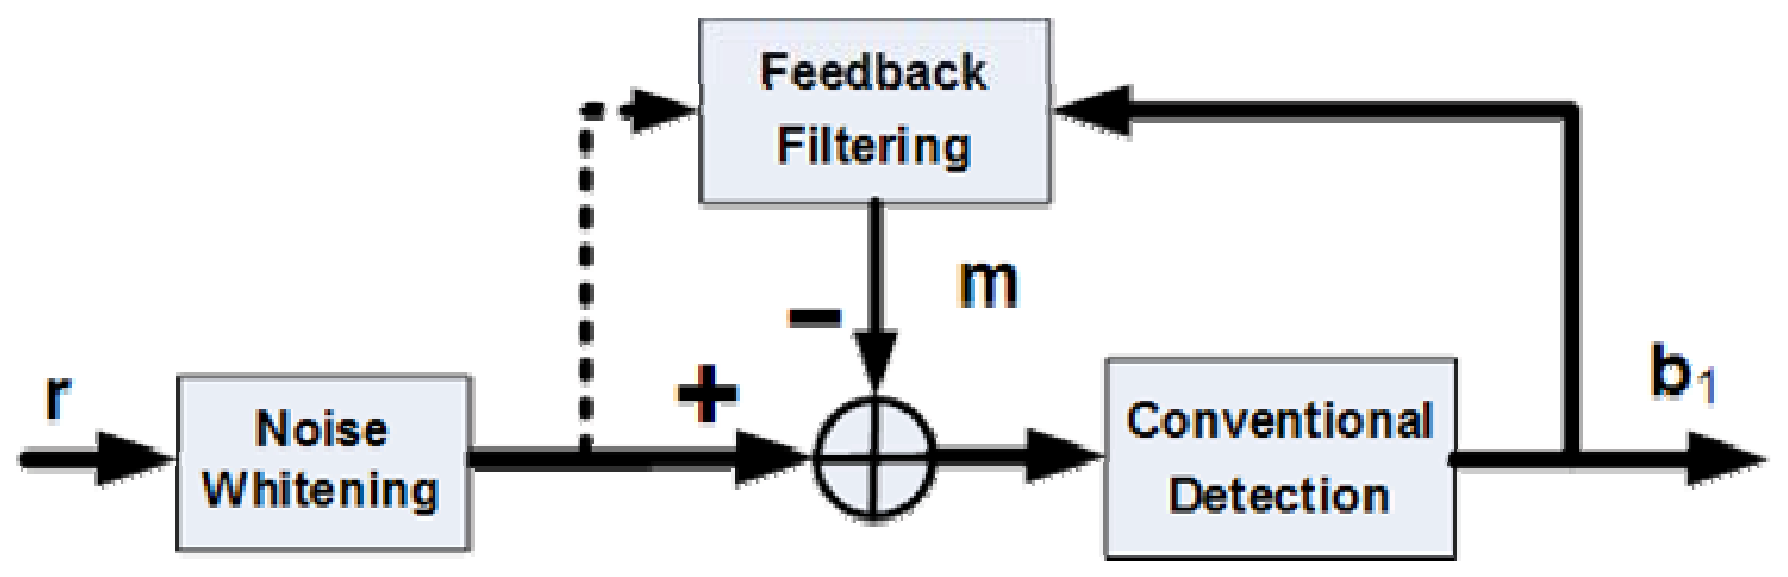
\includegraphics[width=3.2in]{BDFIC1.eps}
\caption{A group-wised decision feedback interference cancellation block diagram} }\label{DFIC}
\end{figure}
Without loss of
the generality, only the signals for the first $G$ known users are detected and their spreading signatures
$\bS_1=\left[\matrix{\bs_1&\bs_2&\ldots&\bs_G}\right]$ are known beforehand. In order to blindly estimate MAI without knowing the original spreading
matrix $\bS$, we define a blind MAI signature matrix
\begin{equation}
\begin{array}{rcl}
\bcS&=&\bigl[\matrix{{\br}[n-1]&{\br}[n-2]&\ldots&{\br}[n-M]}\bigr]\\
&=&\bS\bA\bB+\bN\\
&=&\bS_1\bA_1\bB_1+\bS_2\bA_2\bB_2+\bN
\end{array} \label{bcs}
\end{equation}
\noindent where $\bar\br[n-m]=\br[n-m]-\bS_1\bA_1\bb_1[n-m]$, $m=1,\ 2,\ \ldots,\ M$ and $K\leq M+G\leq L$. $\bB=\bigl[\bB_1^{\rm H}\ \bB_2^{\rm H}\bigr]^{\rm H}$ is the detected data matrix for $\bcS$, $\bS_2$ is the original spreading signature for interfering users,
$\bA_1$, $\bA_2$, $\bB_1$ and $\bB_2$ are the amplitude matrices and data matrices for desired users and interfering users, respectively. $M=K-G$ is the minimum
number for blind interference canceller to unambiguously distinguish
different interfering signals. The relationship between $\bcS$ and $\br$ can be written by
\begin{equation}\hspace{-0.0in}
\begin{array}{rcl}
\br&=&\bigl(\bcS-\bN\bigr)\bB^{+}\bb\\
&=&\bcS\bbf+\tilde{\bn}\ ,
\end{array}\label{brr}
\end{equation}
\noindent where $\bbf=\bB^{+}\bb$ denotes the projection of $\br$ onto the column space of $\bS\bA\bB$, which is similar to $\bS$, $\tilde{\bn}=-\bN\bB^{+}\bb$ and $\left[\cdot\right]^{+}$ denotes the general inverse operation, and the relationship between $\bcS$ and the MAI $\bm$ can be written by
\begin{equation}\hspace{-0.0in}
\begin{array}{rcl}
\bm &=&\bS_2\bA_2\bb_2\\
&=&\bigl(\bcS-\bS_1\bA_1\bB_1-\bN\bigr)\bB_2^{+}\bb_2\\
&=&\bcS\bbf_2-\bS_1\bA_1\bB_1\bbf_2+\tilde{\bn}_2
\end{array}\label{bm}
\end{equation}
\noindent where $\bbf_2=\bB_2^{+}\bb_2$ denotes the projection of $\bm$ onto the column space of $\bS_2\bA_2\bB_2$, which is similar to $\bS_2$, and $\tilde{\bn}_2=-\bN\bB_2^{+}\bb_2$.
With (\ref{bm}), it shows that $\bm$ can be estimated out if $\bbf_2$ is known. However it is not easy to directly estimate $\bbf_2$ from $\bbf$ since they are projected from two different but unorthogonal signal subspaces, respectively.
In order to separate two signal subspaces, a


and $\bm$ can be estimated if $\bbf_2=\bD_2^{+}\bb_2$ is known.

 the first $G$ columns of $\bcS$ and $\bS$ are
same,
\begin{equation}\hspace{-0.0in}
\begin{array}{c}
 \bB=\left[\matrix{\bI_L & \bar\bD\cr\bzero&\tilde\bD }\right]=\left[\matrix{\bE & \matrix{\bar\bD\cr \tilde{\bD}} }\right]
  =\left[\matrix{\bG \cr \matrix{\mathbf{0}& \tilde{\bD}}
 }\right]
\end{array}\label{B}
\end{equation}
\noindent is the $K\times M$ data matrix associated with $\bcS$.
$\bE=[\matrix{\bI_L&\bzero}]^{\rm T}$, $\bG = \left[\matrix{\bI_L&
\bar\bD}\right]$ is the $G\times M$ matrix composed by known data
in $\bcS$. $\mbox{rank}\{\tilde{\bD}\}=K-G$ and
$\mbox{rank}\{\bB\}\leq K$.

After the blind spreading matrix $\bcS$ is defined, the received
signal vector $\br$ in (\ref{r_sync}) can be expressed as the
linear combination of the columns in $\bcS$ instead of $\bS$ by
\begin{equation}
\begin{array}{rcl}
\br&=&\bcS\bbf + \bar{\bn}\label{r_blind}
\end{array}
\end{equation}
\noindent where the $M \times 1$ vector $\bbf$ is termed the
detection vector defined by
\begin{equation}
\begin{array}{rcccl}
\bbf&=&\left[\matrix{\bbf_1\cr\bbf_2}\right]&=&\bB^{+}\bar\bb
\end{array} \label{DetectorVector}
\end{equation}
\noindent where $\bbf_1$ is the subvector of $\bbf$ consisting of
the first $G$ elements of, $\bbf_2$ consists of the rest $M-G$
elements, $[\cdot]^{+} $ denotes the general inverse operator and
$\bar\bb=\bA \bb$. $\bar{\bn}$ is the new $L\times 1$ noise vector
defined by
\begin{equation}
\begin{array}{rcl}
\bar{\bn}&=&\bn-{\bN}\bB^{+}\bar\bb
\end{array}. \label{new_noise}
\end{equation}
\noindent Meanwhile, the MAI part of $\br$ can be written by
\begin{equation}
\begin{array}{rcccl}
\bm&=&\bS_2\bA_2\bb_2 &=&\left(\bcS_2-\bcS_1\bar\bD\right)\bbf_2
\end{array}
\end{equation}
\noindent where $\bS_2$, $\bA_2$ and $\bb_2$ denote the original
spreading sequences, amplitudes and information bits for
interfering users. In order to separate MAI from received signal
for estimating $\bbf_2$, we perform QR-decomposition on $\bS_1$ by
\begin{equation}
\begin{array}{rcl}
\bS_1&=&\bQ_1\bR_1
\end{array},
\end{equation}
\noindent where $\bQ_1\in\mathbb{R}^{L\times L}$ is orthogonal and
$\bR_1=[\bR_{11}^{\rm H}\ \bzero^{\rm H}]^{\rm
H}\in\mathbb{R}^{L\times G}$, and apply $\bQ_1^{\rm H}$ on both
sides of (\ref{r_sync}) and (\ref{r_blind}). We then get
\begin{equation}
\begin{array}{rcl}
\bQ_{1}^{\rm
H}\br&=&\left[\matrix{\bR_{11}\bA_1\bb_1\cr\bzero}\right]+\left[\matrix{\bR_{12}\bA_2\bb_2\cr\bR_{22}\bA_2\bb_2}\right]+\bQ_1^{\rm
H}\bn\\
&=&\left[\matrix{\bcR_{11}\bbf_1\cr\bzero}\right]+\left[\matrix{\bcR_{12}\bbf_2\cr\bcR_{22}\bbf_2}\right]+\bQ_1^{\rm
H}\bar\bn
\end{array}
\end{equation}
\noindent where the matrices $\bR_{11}$, $\bR_{12}$ and $\bR_{22}$
are given by
\begin{equation}
\begin{array}{rcl}
\bQ_{1}^{\rm
H}\bS&=&\left[\matrix{\bR_{11}&\bR_{12}\cr\bzero&\bR_{22}}\right]
\end{array}
\end{equation}
\noindent and the matrices $\bcR_{11}$, $\bcR_{12}$ and
$\bcR_{22}$ are given by
\begin{equation}
\begin{array}{rcl}
\bQ_{1}^{\rm
H}\bcS&=&\left[\matrix{\bcR_{11}&\bcR_{12}\cr\bzero&\bcR_{22}}\right]
\end{array}.
\end{equation}
Now we can see that $\bbf_2$ can be estimated with solving
\begin{equation}\hspace{-0.05in}
\begin{array}{rcl}
\bT\bQ_{1}^{\rm H}\br&=&\bcR_{22}\bbf_2+\bT\bQ_1^{\rm H}\bar\bn
\end{array},\label{f2}
\end{equation}
\noindent where $\bT=\left[\matrix{\bzero&\bI_{L-G}}\right]$ is
termed truncating matrix.

\noindent After $\bbf_2$ is estimated, the MAI $\bm$ can be
estimation using (\ref{bm}) and cancelled so that $\bb_1$ can be
detected with solving
\begin{equation}
\begin{array}{l}
\hat{\bb}_1=\mbox{arg}\min\limits_{\bb_1}\left\|\bS_1\bA_1\bb_1-\left[\br-\left(\bcS_2-\bcS_1\bar\bD\right)\hat{\bbf}_2\right]\right\|_2^2
\end{array}\label{br_bm}
\end{equation}
\noindent or
\begin{equation}
\begin{array}{l}
\hat{\bb}_1=\mbox{arg}\min\limits_{\bb_1}\mbox{E}\left\|\bS_1\bA_1\bb_1-\left[\br-\left(\bcS_2-\bcS_1\bar\bD\right)\hat{\bbf}_2\right]\right\|_2^2
\end{array}\label{br_bm}
\end{equation}


\subsection{Least Square IC}
In least square interference cancellation approaches, both the
interference $\bm$ and $\bb_1$ are estimated and detected with
least square criterion. After $\bbf_2$ is estimated, the
interference cancellation can be performed using
\begin{equation}\hspace{-0.1in}
\begin{array}{l}
\hat{\bb}_1=\mbox{sgn}\left\{\mbox{arg}\min\limits_{\by}\left\|\br-\left(\bcS_2-\bcS_1\bar\bD\right)\hat{\bbf}_2-\bS_1\bA_1\by\right\|_2\right\}
\end{array}.
\end{equation}
There are typically two approaches for estimating $\bbf_2$ with
least square criterion. One is the classic least-square approach,
which can be expressed by
\begin{equation}\hspace{-0.10in}
\begin{array}{rcl}
\hat{\bbf}_2^{\rm
LS}&=&\mbox{arg}\min\limits_{\bx}\left\|\bT\bQ_{1}^{\rm
H}\br-\bcR_{22}\bx\right\|_2\\
&=&\bcR_{22}^{+}\bT\bQ_{1}^{\rm H}\br\ .
\end{array}
\end{equation}
\noindent The LS-IC for the first $G$ users can then be written by
\begin{equation}\hspace{-0.02in}
\begin{array}{l}
\hat{\bb}_{1}^{\rm
LS}=\mbox{sgn}\left\{\bS_{1}^{+}\br-\bS_{1}^{+}\left(\bcS_{2}-\bcS_{1}\bar{\bD}\right)\bcR_{22}^{+}\bT\bQ_{1}^{\rm
H}\br\right\}
\end{array}\label{b_LS_IC}
\end{equation}
\noindent Another one is the total-least-square (TLS) approach,
which can be expressed by
\begin{equation}\hspace{-0.08in}
\begin{array}{rcl}
\left[\matrix{\hat{\bcR}_{22}\cr\hat{\bbf}_2^{\rm
TLS}}\right]&=&\mbox{arg}\min\limits_{\bY\
\bx}\left\|\left[\matrix{\bcR_{22}\cr\bT\bQ_{1}^{\rm
H}\br}\right]-\left[\matrix{\bY\cr\bY\bx}\right]\right\|_2
\end{array}.
\end{equation}
\noindent If $\sigma_{K-G}'>\sigma_{K-G+1}$, the TLS estimation of
$\bbf_2$ is
\begin{equation}\hspace{-0.070in}
\begin{array}{rcl}
{\bbf_2^{\rm TLS}}&=&\left(\bcR_{22}^{\rm
H}\bcR_{22}-\sigma_{K-G+1}^{2}\bI\right)\bcR_{22}^{\rm
H}\bT\bQ_{1}^{\rm H}\br
\end{array}
\end{equation}
\noindent where $\sigma_{K-G}'$ and $\sigma_{K-G+1}$ are the
$(K-G)$th and $(K-G+1)$th largest singular value of $\bcR_{22}$
and $\left[\matrix{\bT\bQ_{1}^{\rm H}\br&\bcR_{22}}\right]$. And
the TLS-IC can be expressed by
\begin{equation}\hspace{0.0in}
\begin{array}{l}
\hat{\bb}_{1}^{\rm
TLS}=\mbox{sgn}\left\{\bS_{1}^{+}\br-\bS_{1}^{+}\left({\bcS}_{2}-{\bcS}_{1}{\bar{\bD}}\right){\bbf_2^{\rm
TLS}}\right\}
\end{array}\label{b_TLS_IC}
\end{equation}

\subsection{Minimum Mean-Square Error IC}
In MMSE-based approach,the interference cancellation is done with
solving
\begin{equation}\hspace{-0.1in}
\begin{array}{l}
\hat{\bb}_1=\mbox{sgn}\left\{\mbox{arg}\min\limits_{\by}\mbox{E}\left\|\br-\left(\bcS_2-\bcS_1\bar\bD\right)\hat{\bbf}_2-\bS_1\bA_1\by\right\|_2\right\}\
,
\end{array}
\end{equation}
\noindent providing $\bbf_2$ is estimated. On the other hand,
$\bbf_2$ is estimated with minimizing MSE
\begin{equation}\hspace{-0.08in}
\begin{array}{rcl}
\hat{\bbf}_2^{\rm
MMSE}&=&\mbox{arg}\min\limits_{\bx}\mbox{E}\left\|\bT\bQ_{1}^{\rm
H}\br-\bcR_{22}\bx\right\|_2^2\\
&=&\left(\bcR_{22}^{\rm
H}\bcR_{22}-\sigma^2\bI\right)^{-1}\bcR_{22}^{\rm
H}\bT\bQ_{1}^{\rm H}\br
\end{array}
\end{equation}
\noindent so that the MMSE-IC can be written by
\begin{equation}\hspace{-0.10in}
\begin{array}{l}
\hat{\bb}_1=\mbox{sgn}\left\{\left(\bS_1\bA_1^2\bS_1^{\rm
H}-\sigma^2\bI\right)\bS_1^{\rm
H}\left(\br-\left(\bcS_2-\bcS_1\bar\bD\right)\hat{\bbf}_2\right)\right\}
\end{array}.
\end{equation}


\section{Performance Analysis}

\subsection{Relationship with Blind MUD}

It can be proven that the LS-IC in (\ref{b_LS_IC}) actually is
equal to a blind LS decorrelating detector
\begin{equation}
\begin{array}{rcl}
\hat{\bb}_{1}&=&\mbox{sgn}\left\{\bG\bbf_{\rm LS}\right\}
\end{array}
\end{equation}
\noindent with respect to
\begin{equation}
\begin{array}{rcl}
{\bbf}_{\rm
LS}&=&\matrix{\mbox{arg}\min\limits_{\bx}\left\|\br-\bcS\bx\right\|_2}
\end{array}
\label{LSProb}
\end{equation}
\noindent and MMSE-IC is the same to the blind MMSE detector
\begin{equation}\hspace{0.0in}
\begin{array}{rcl}
\hat{\bb}_1&=&\mbox{sgn}\left\{\bG\bbf_{\rm MMSE}\right\}
\end{array}
\end{equation}
\noindent with respect to
\begin{equation}
\begin{array}{rcl}
{\bbf}_{\rm
MMSE}&=&\mbox{arg}\min\limits_{\bx}E\left\{\left\|\bbf-\bx\right\|_2^2\right\}
\end{array}.
\end{equation}

\subsection{AME and Near-Far Resistance}
A commonly used performance measure for a multiuser detector is
asymptotic multiuser efficiency (AME) and near-far
resistance~\cite{Verd98}. Since the proposed algorithms converges
to the conventional decorrelating detector as $\sigma^2\rightarrow
0$, their AME and near-far resistance are identical to the
decorrelating detector:
\begin{equation}
\begin{array}{rcl}
\bar{\eta}_k&=&\frac{1}{\left[\bR^{+}\right]_{kk}}
\end{array}.
\end{equation}
\subsection{CRLB for $\bbf_2$ Estimation}
The Cram\'{e}r-Rao Lower Bound (CRLB) is given by the inverse of
the Fisher information matrix (FIM). Providing the blind spreading
matrix $\bcS$ is known beforehand, we first define the parameter
vector $\mathbf{\phi} = \left[\bar{\sigma}^{2}\ \bbf_2^{\rm
H}\right]^{\rm H}$, where $\bar{\sigma}^{2}
=(1+\frac{M-G}{M-K})\sigma^{2}$, for computing the FIM
\begin{equation}
\begin{array}{rcl}
{\bI(\mathbf{\phi})} &=& {\rm E} \left\{ \left( \frac{\partial
\ln{\cal L}}{\partial \mathbf{\phi}} \right) \left( \frac{\partial
\ln{\cal L}}{\partial \mathbf{\phi}} \right)^{\rm H} \right\}
\label{fim}
\end{array}
\end{equation}
\noindent where $\ln{\cal L}$ is the log-likelihood function given
by
\begin{equation}
\begin{array}{rcl}
\ln{\cal
L}&=&C-L\ln\bar{\sigma}^2-\frac{1}{2\bar{\sigma}^2}\parallel\mathbf{e}\parallel_2^2
\end{array},\label{logl}
\end{equation}
\noindent $C$ is a constant and
$\mathbf{e}=\bT\bQ_1\br-\bcR_{22}\bbf_2$. Providing $\bcS$ is
known, the closed-form CRLB expression of $\bbf_2$ is then given
by
\begin{equation}
\begin{array}{rcl}
{\rm CRLB}(\bbf_2\ |\ \bcS) &
=&(1+\frac{M-G}{M-K})\sigma^{2}(\bcR_{22}^{\rm H}\bcR_{22})^{\rm
+}
\end{array}.\label{CRLB_f}
\end{equation}
\noindent It shows that the accuracy of estimating $\bbf_2$ may
increase with increasing $M$.
\subsection{Bit-Error Rate}

\section{Computer Simulations}
There are $K=10$ users with the group size $G=3$ and the spreading
sequences used in simulations are $64$-chip ($L=64$) random
sequences. In the computer simulations, the previous amplitude
estimation from (\ref{A_estimation}) is directly use for the next
detection without any amplitude filtering. From Subplot (a) in
Fig. 3, it is interesting to see that the performance of the
simplest LS detector has the best performance. From Subplot (b),
it is very impressive to find that the performance of blind LS
detector is very close to the conventional decorrelating detector
whatever how strong the MAI is in our simulations when $M$ is
large enough. We then check the performance of the proposed LS
blind detector against the amplitude estimation errors. From Fig.
4, we can see that the BER of the LS detector basically is
unchanged against amplitude estimation error when SNR is large
enough. From Fig. 5, we can see that the performance of the LS
detector can be better providing $M$ is larger enough. This
confirms (\ref{noise_var_new}), which shows that the variance of
$\bar{\bn}$ decrease with increasing $M$.
\begin{figure} \center{
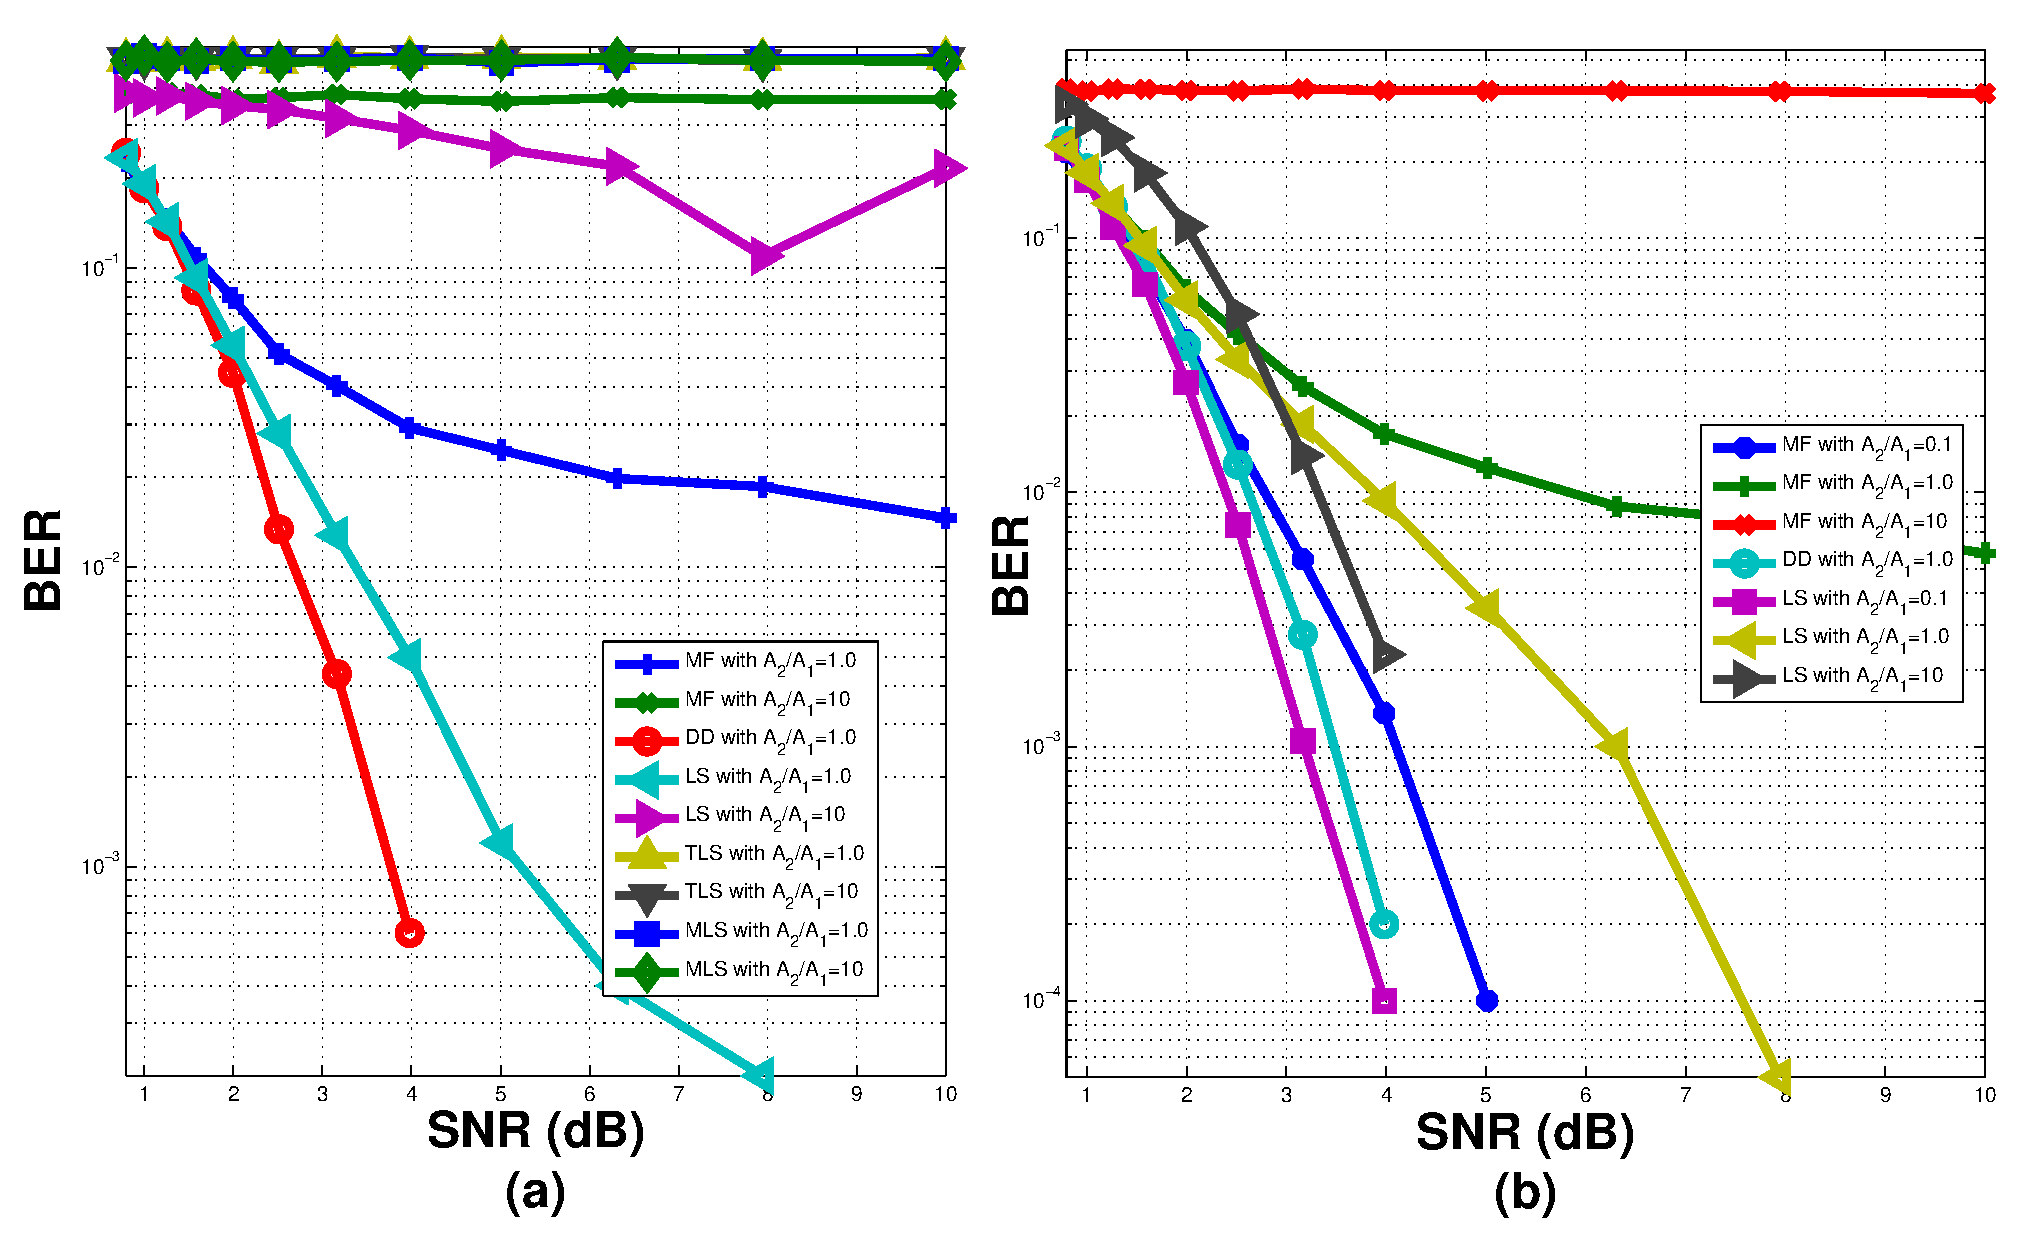
\includegraphics[width=3in]{BER_SNR_10_64.eps}
\caption{ (a) The performance of the proposed blind MUDs against
SNR, $M=12$. (b) The performance of the proposed blind LS
detector, $M=63$. } }\label{BER_SNR}
\end{figure}
\begin{figure} \center{
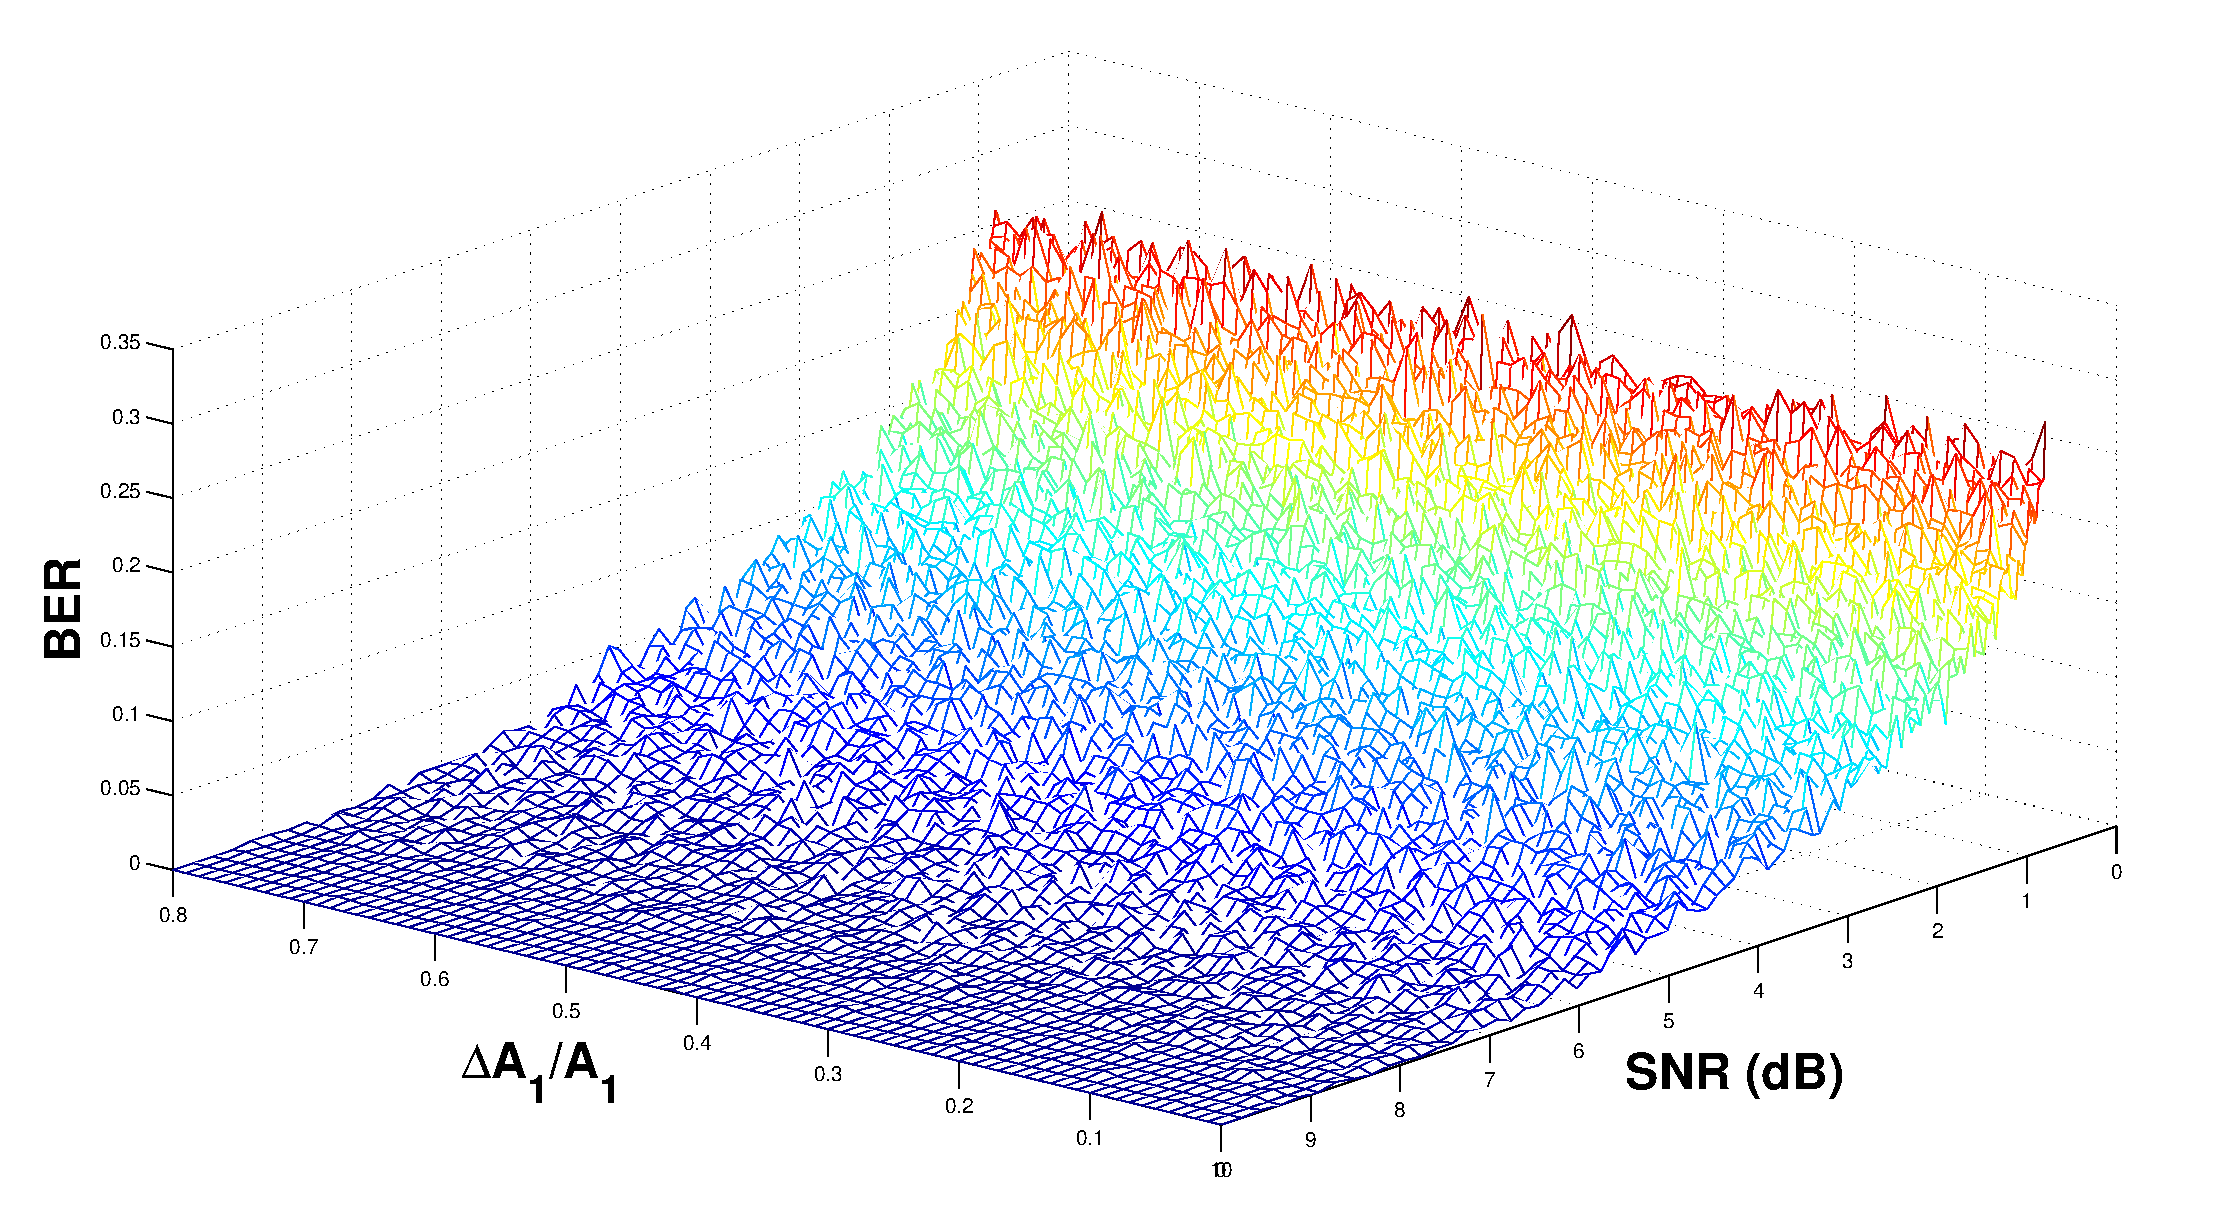
\includegraphics[width=2.5in]{BER_A_SNR_10_64_LSs.eps}
\caption{ The performance of the LS detector against amplitude
estimation error ${\Delta}{A_1}/A_1$ and SNR, $M=63$.}
}\label{BER_A_SNR}
\end{figure}
\begin{figure}
\center{
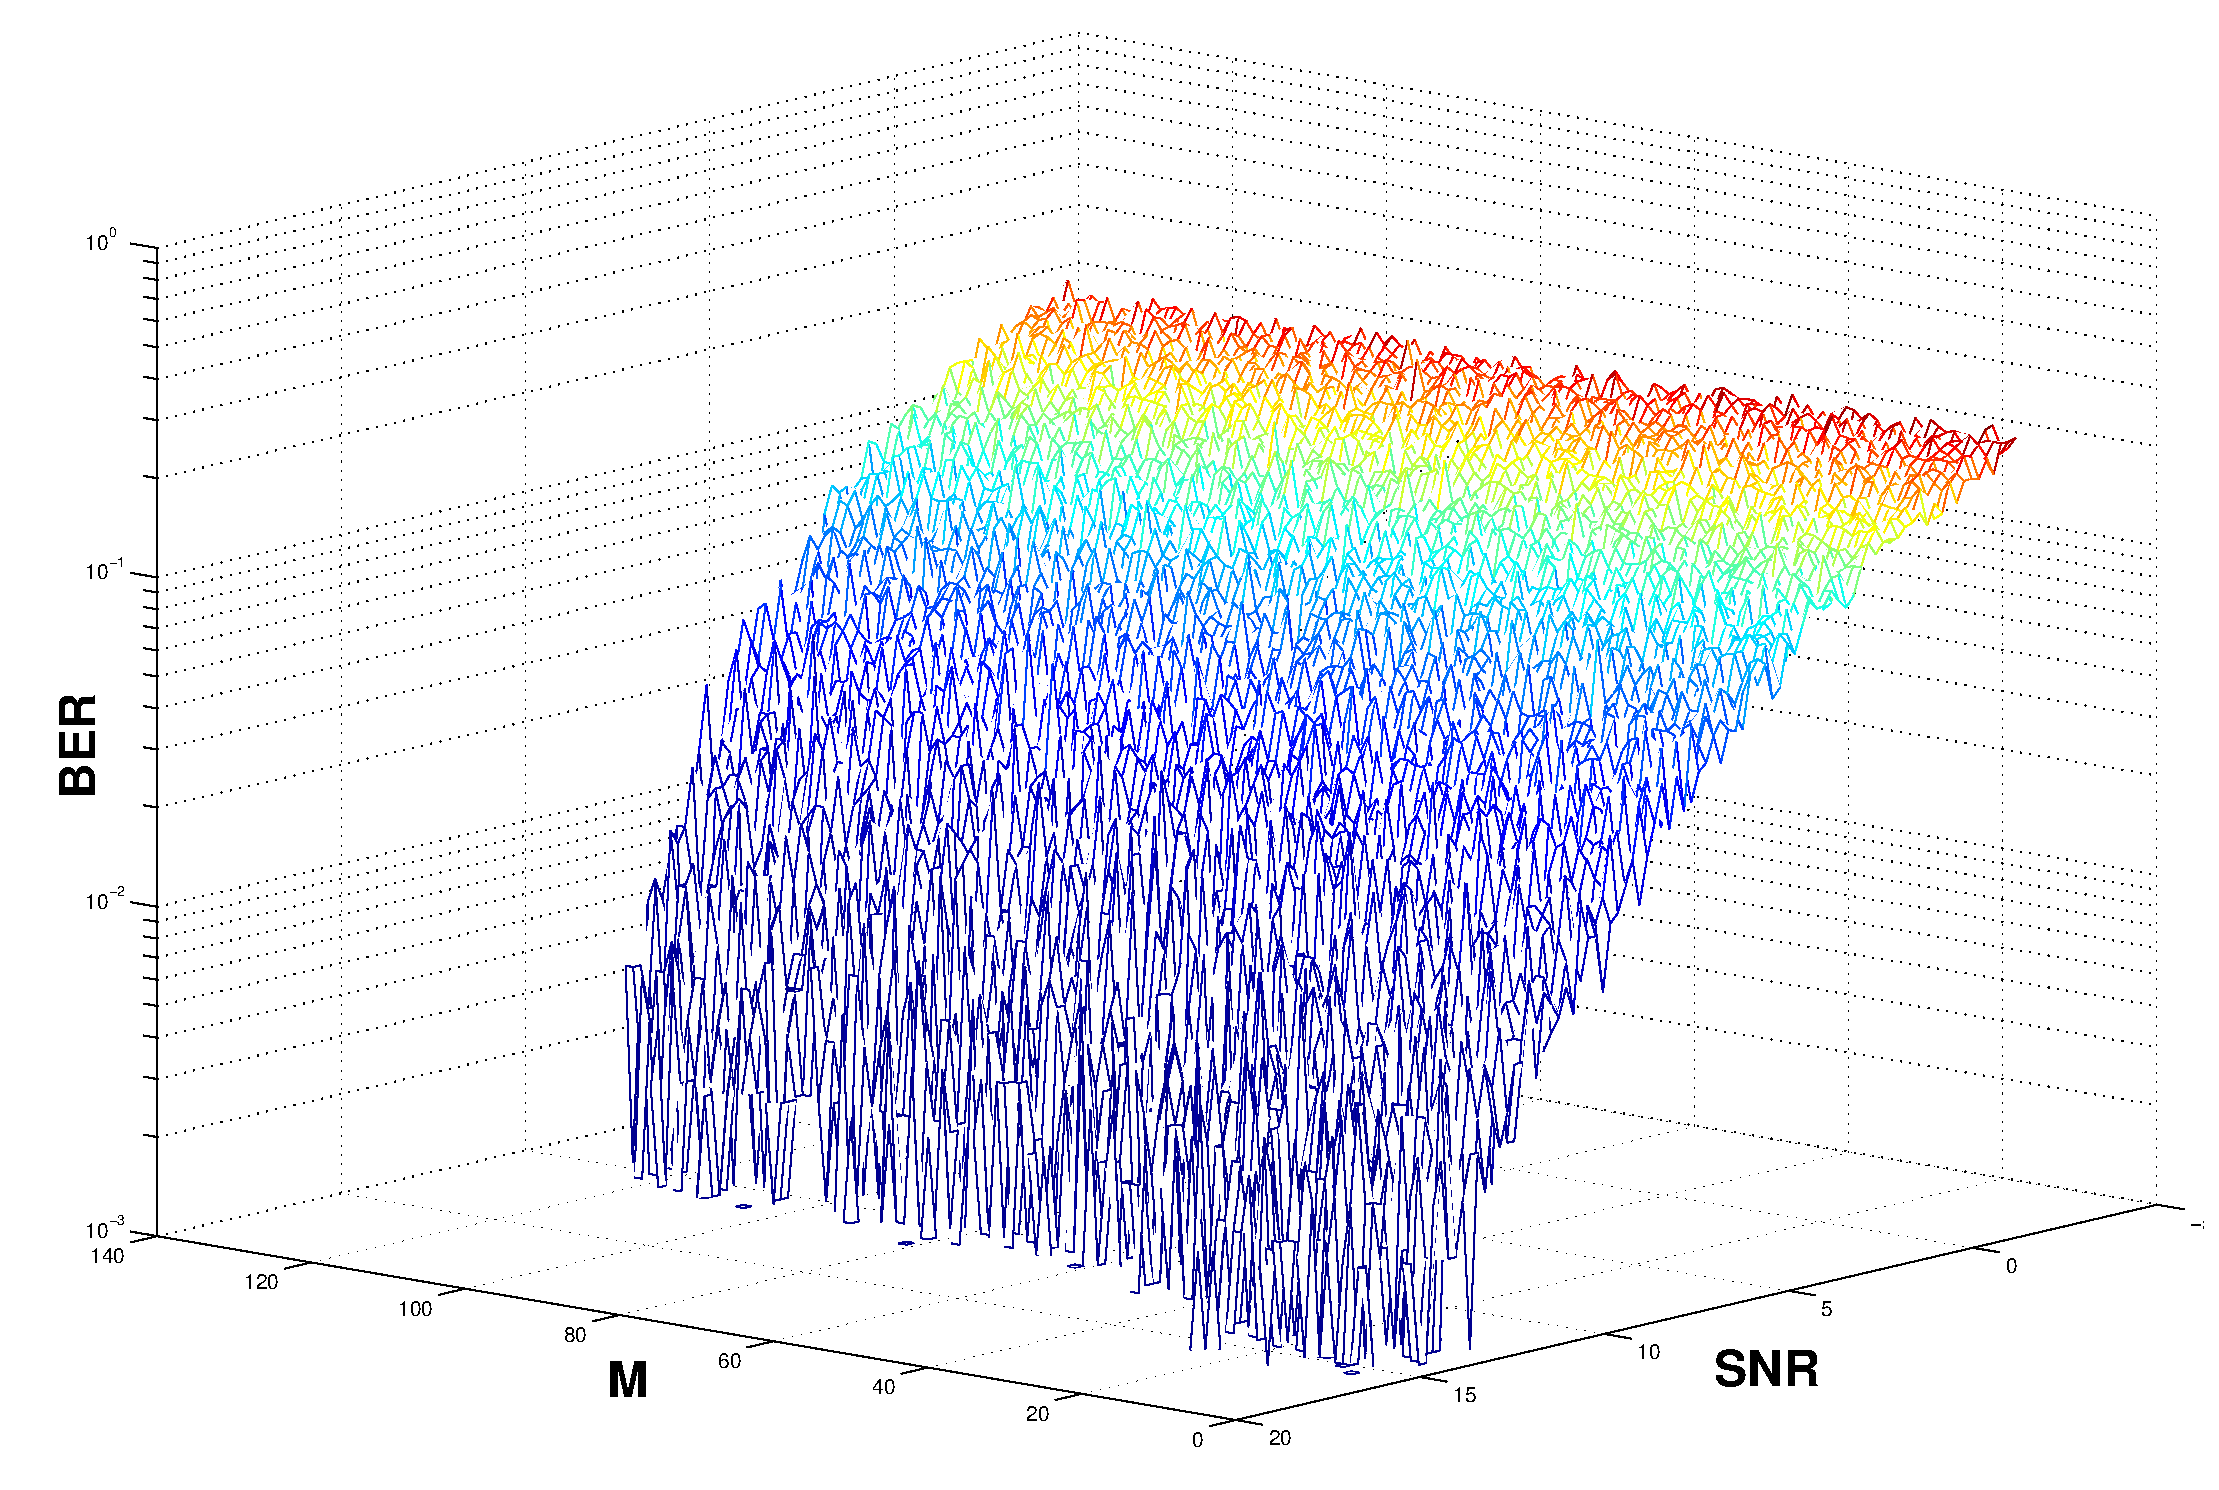
\includegraphics[width=2.5in]{BER_M_SNR_10_64_LSs.eps}
\caption{ The performance of the LS blind MUD against $M$ and
SNR.} }\label{BER_M_SNR}
\end{figure}
\section{Conclusions}
In this paper, we proposed a blind multiuser detection framework
as well as several blind detectors. The proposed blind detectors
are direct and simple without any channel or spreading sequence
estimation or subspace separation operation.
\small
\bibliographystyle{unsrt}
\bibliography{FastBDD,InterferenceCancellation}
\end{document}
